\documentclass[ucs, notheorems, handout]{beamer}

\usetheme[numbers,totalnumbers,minimal,nologo]{Statmod}
\usefonttheme[onlymath]{serif}
\setbeamertemplate{navigation symbols}{}
\setbeamercolor{alerted text}{fg=blue}
\usepackage{physics}

\mode<handout> {
    \usepackage{pgfpages}
    %\setbeameroption{show notes}
    %\pgfpagesuselayout{2 on 1}[a4paper, border shrink=5mm]
    \setbeamercolor{note page}{bg=white}
    \setbeamercolor{note title}{bg=gray!10}
    \setbeamercolor{note date}{fg=gray!10}
}

\usepackage[utf8x]{inputenc}
\usepackage[T2A]{fontenc}
\usepackage[english, russian]{babel}
\usepackage{tikz}
\usepackage{ragged2e}
\usepackage{graphicx}
\usepackage{subfigure}


\usepackage{latexsym,amssymb}
\usepackage{amsmath}
\usepackage{amsfonts}
\usepackage{amsthm}

\DeclareMathOperator{\rk}{rk}
\DeclareMathOperator{\med}{med}
\DeclareMathOperator{\diag}{diag}
\DeclareMathOperator*{\argmin}{argmin}
\newcommand{\tX}[1]{\mathsf{#1}}
\newcommand{\iu}{{i\mkern1mu}}

\title[Комплексные выбросы и SSA]
{Ошибки оценивания сигнала с помощью комплексного анализа сингулярного спектра}

\subtitle
{}

\author[Сенов М.А.] 
{Сенов Михаил Андреевич}

\institute[Санкт-Петербургский Государственный Университет]{%
    \small
    Санкт-Петербургский государственный университет\\
    Прикладная математика и информатика\\
    Вычислительная стохастика и статистические модели\\
    \vspace{1.25cm}
    Отчет по научно-исследовательской работе}

\date[Зачет]{Санкт-Петербург, 2022}

\begin{document}

\begin{frame}
  \titlepage
  \note{}
\end{frame}

\begin{frame}{Введение: Проблема}

$\tX{X} = (x_1, \ldots, x_{N})$ временной ряд длины $N$.\\
\vspace{1em}
\alert{Модель:} $\tX{X} = \tX{S} + \tX{R}$, $\tX{S}$ сигнал, $\tX{R}$ возмущение.\\
\vspace{1em}
\alert{Проблема:} Извлечение сигнала $\tilde{\tX{S}} = F(\tX{X})$, $F$ используемый метод.\\
\vspace{1em}
\alert{Метод:} SSA (Singular Spectrum Analysis) [Analysis of Time Series
Structure: SSA and Related Techniques, Golyandina N., Nekrutkin V.,
Zhigljavsky A., 2001].

    \note{}
\end{frame}

\begin{frame}{Введение: Ошибка восстановления}
    \alert{Модель:} $\tX{S}(\delta) = \tX{S} + \delta \tX{R}$ длины $N$\\
    или\\
     $\mathbf{H}(\delta) = \mathbf{H} + \delta \mathbf{E}$, где $\mathbf{H}(\delta) = \mathcal{T}(\tX{S}(\delta))$, $\mathbf{H} = \mathcal{T}(\tX{S})$, $\delta\mathbf{E} = \mathcal{T}(\delta \tX{R})$, $\mathcal{T}$~--- оператор ганкелизации.\\
     $\mathbf{P}_k$~--- проектор на $k$-ое ортогональное собственное пространство $\mathbf{H}\mathbf{H}^{\mathrm{H}}$.\\
     $\mathbf{P}_k(\delta) = \mathbf{P}_k + \delta\mathbf{P}^{(1)}_k +  \delta^2\mathbf{P}^{(2)}_k + \ldots$\\
     $\mathbf{H}_k(\delta) = \mathbf{P}_k(\delta) \mathbf{H} = \mathbf{H}_k + \delta\mathbf{H}^{(1)}_k +  \delta^2\mathbf{H}^{(2)}_k + \ldots$\\
     \vspace{1em}
     $\mathbf{H}^{(1)} = \sum_{i = 1}^{r} \mathbf{H}^{(1)}_i$\\
     $\tX{F}^{(1)} = \mathcal{H}(\mathbf{H}^{(1)})$ первый порядок ошибки восстановления.\\
     \vspace{1em}
    
\end{frame}

\begin{frame}{Ошибка восстановления: Формула для $\mathbf{H}^{(1)}$}
На основе результатов из (Константинов, 2018) и (Некруткин, 2015) была получена формула для $\mathbf{H}^{(1)}$ в случае достаточно маленького возмущения.

\begin{equation*} \label{eq:main}
	\mathbf{H}^{(1)} = \mathbf{P}_0 \mathbf{E} \mathbf{Q}^{\perp}_0 + \mathbf{P}^{\perp}_0 \mathbf{E},
\end{equation*}
где $\mathbf{P}^{\perp}_0$~--- проектор на пространство столбцов $\mathbf{H}$, $\mathbf{Q}^{\perp}_0$~--- проектор на пространство строк $\mathbf{H}$, $\mathbf{P}_0 = \mathbf{I} - \mathbf{P}^{\perp}_0$, $\mathbf{I}$~--- единичная матрица.
\end{frame}

\begin{frame}{Ошибка восстановления: Теорема}
    $\tX{F}^{(1)} = (f^{(1)}_1, \ldots, f^{(1)}_N)$ первый порядок ошибки восстановления $\tX{S}$ с возмущением $\tX{R}$ метода CSSA,

    $\tX{F}^{(1)}_{\Re} = (f^{(1)}_{\Re,1}, \ldots, f^{(1)}_{\Re, N})$ первый порядок ошибки восстановления $\Re(\tX{S})$ с возмущением $\Re(\tX{R})$ метода SSA,

    $\tX{F}^{(1)}_{\Im} = (f^{(1)}_{\Im,1}, \ldots, f^{(1)}_{\Im, N})$ первый порядок ошибки восстановления $\Im(\tX{S})$ с возмущением $\Im(\tX{R})$ метода SSA.
    
    \begin{block}{Теорема \label{th:sum}}
        Пусть пространства столбцов траекторных матриц рядов $\tX{S}$, $\Re(\tX{S})$ и $\Im(\tX{S})$ совпадают и то же самое верно для пространств строк.
    Тогда при любом достаточно малом возмущении $\tX{R}$ 
    $$\tX{F}^{(1)} = \tX{F}^{(1)}_{\Re} + \iu\tX{F}^{(1)}_{\Im}.$$
    \end{block}
    Получается из линейности вхождения $\mathbf{E}$ в формулу для $\mathbf{H}^{(1)}$.
\end{frame}

\begin{frame}{Ошибка восстановления: Случайное возмущение}
    $\tX{R}$~--- случайный вектор.\\
    \vspace{1em}
    \alert{Известно:} Пусть $\zeta = \xi + \iu\eta$. Тогда $\mathbb{D}(\zeta) = \mathbb{D}(\xi) + \mathbb{D}(\eta)$.
    \begin{block}{Следствие (из теоремы)}
        Пусть выполнены условия теоремы.
	
	Тогда
	\begin{equation*} \label{eq:dispsum}
	\mathbb{D}f^{(1)}_l = \mathbb{D}f^{(1)}_{\Re, l} + \mathbb{D}f^{(1)}_{\Im, l}.	
	\end{equation*}
    \end{block}
    Получается автоматически из теоремы и известного результата.
    
\end{frame}

\begin{frame}{Две зашумлённые синусоиды: Модель}
Пусть сигнал $\tX{S}$ имеет вид
\begin{equation*}
\label{eq:general_ts}
s_l = A\cos(2 \pi\omega l + \phi_1) + \iu B\cos(2 \pi\omega l + \phi_2),
\end{equation*}
где $0<\omega\le 0.5$ и $0\le\phi_i < 2\pi$.

При $|\psi_2-\psi_1| = \pi/2$ и $A=B$, 
$$s_l = e^{i(2 \pi\omega l + \phi_1)}.$$
Пусть возмущение $\tX{R}$~--- шум, т.е. случайный вектор с нулевым матожиданием и достаточно малой дисперсией.

\end{frame}

\begin{frame}{Две зашумлённые синусоиды: MSE}
\begin{block}{Замечание}
    Для сигнала $s_l$, $s_l \neq e^{i(2 \pi\omega l + \phi_1)}$ с возмущением $\tX{R}$ выполняется формула разложения дисперсии из следствия.
\end{block}

Совпадение пространств для $s_l$ известно из (Степанов,~Голяндина,~2005).

Для сигнала $s_l = e^{i(2 \pi\omega l + \phi_1)}$ численно было показано поточечное равенство MSE CSSA-оценок полусумме MSE SSA-оценок вещественной и мнимой части. 

\end{frame}

\begin{frame}{Константный сигнал с выбросом: Модель и вид $\mathbf{H}^{(1)}$}
Пусть сигнал $\tX{S}$ имеет вид
$$s_l = c_1 + \iu c_2.$$
Пусть возмущение $\tX{R} = (0, \ldots, a_1 + \iu a_2, \ldots, 0)$~--- выброс на позиции $k$.

По теореме достаточно выразить $\tX{F}^{(1)}_{\Re}$.

Для вещественных рядов с $\rk(\mathbf{H}) = 1$ известна формула (Nekrutkin, 2008).
$$\mathbf{H}^{(1)} = -U^{\mathrm{T}} \mathbf{E} V U V^{\mathrm{T}} + U U^{\mathrm{T}} \mathbf{E} + \mathbf{E} V V^{\mathrm{T}},$$
где $U$, $V$~--- сингулярные вектора матрицы $\mathbf{H}$.

Подставляем  $U = \{1/\sqrt{L}\}^{L}_{i = 1},\, V = \{1/\sqrt{K}\}^{K}_{i = 1}$, $K = N - L + 1$.
\end{frame}

\begin{frame}{Константный сигнал с выбросом: Явный вид $f^{(1)}_l$}
    Приведем результат для случая $k \leq \min(L/2, K - L)$ и $L < K$
$$f^{(1)}_l = \frac{a}{{LK}}
\begin{cases}
	(L + K - k), & \text{$1 \leq l \leq k$}\\
	\frac{1}{l}(L + K - l)k, & \text{$k < l \leq L$}\\
	\frac{1}{L}K(L + k - l), &\text{$L < l < L + k$}\\
	0, &\text{$L + k \leq l \leq K$}\\
	\frac{1}{N - l + 1}(K - l)(L - k), &\text{$K < l < K + k$}\\
	-k, &\text{$K + k \leq l \leq N $}
\end{cases}.$$

\alert{Замечание:} При фиксированном $L$ первый порядок ошибки не стремится к $0$ с ростом $N$.
\end{frame}

\begin{frame}{Сравнение первого порядка и полной ошибок: Зашумлённые гармоники}
Рассмотрим
$$s_l = \cos(2 \pi l / 10) + \iu\cos(2 \pi l / 10 + \pi/4),$$
$\tX{R}$~--- белый шум с $\sigma^2 = 0.1$, $N = 49$, $L = 5$.
\begin{figure}[H]
	\begin{center}
		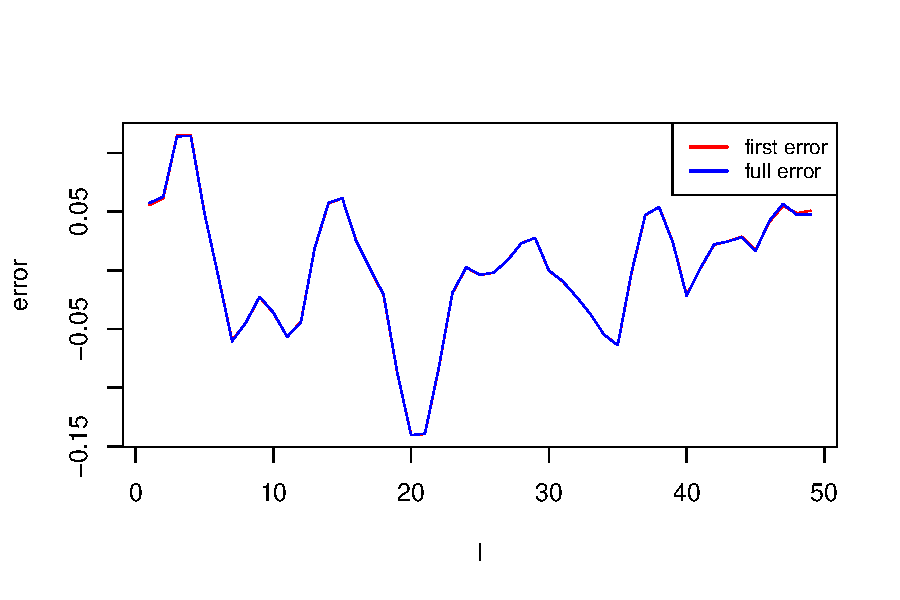
\includegraphics[width=0.6\linewidth]{first_vs_full_re.png}
		\caption{Вещественные части первого порядка и полной ошибок.}
		\label{fig:harm_noise}
	\end{center}
\end{figure}
\alert{Вывод:} Первый порядок почти совпадает с полной ошибкой.
\end{frame}

\begin{frame}{Сравнение первого порядка и полной ошибок: Константный сигнал с выбросом}

Рассмотрим
$$s_l = 1 + \iu,$$
$\tX{R}$~--- выброс $10 + \iu 10$ на позиции $k = L - 1$.

\begin{table}[H]
	\begin{center}
		\caption{Максимальное различие первого порядка и полной ошибок.}
		\label{tab:const_outl}
		\begin{tabular}{|c|c|c|c|c|}
			\hline
			$N$	& 50 & 100 & 400 & 1600 \\
			\hline
			$L = N / 2$ & 0.1313  & 0.0419  & 0.0033 & 0.0002 \\
			\hline
			$L = 20$ & 0.3074  & 0.1965  & 0.5655 & 0.6720 \\
			\hline
		\end{tabular}
	\end{center}
\end{table}

\alert{Вывод:} Первый порядок адекватно оценивает полную ошибку только в случае, когда $L$ и $K$ пропорциональны $N$.

\end{frame}

\begin{frame}{Заключение}
    \begin{itemize}
        \item Подведена теоретическая база под имеющиеся численные результаты (Golyandina et al., 2013) для случая зашумлённых гармоник со сдвигом, не равным $\pi / 2$.
        \item Для случая комплексной экспоненты известный численный результат был обобщён.
        \item Результаты показывают, что применение CSSA имеет смысл только для случая комплексной экспоненты.
        \item Для константного ряда с выбросами был получен явный вид первого порядка ошибки в каждой точке.
        \item Для обоих случаев было численно исследовано соотношение между первым порядком ошибки и полной ошибкой.  
    \end{itemize}
\end{frame}


\end{document}
